\documentclass[pdftex,11pt,a4paper]{article}
\usepackage[pdftex]{graphicx}
\usepackage{fancyhdr}
\usepackage{geometry}
\usepackage{draftcopy}
\usepackage{float}
\usepackage{amsmath}
\usepackage{algorithm2e}

\renewcommand{\thesection}{\arabic{section}.}
\renewcommand{\thesubsection}{\arabic{section}.\arabic{subsection} }
\renewcommand{\headrulewidth}{0pt}
\renewcommand{\footrulewidth}{0.5pt}
\pagestyle{fancy}
\fancyhead{}
\fancyfoot[LE,LO]{\footnotesize{
SE344, Chemistry and Our Environment
}
}

\title{\vspace{-15pt}Biodegradability and Metabolism of Aromatics\\ SE344: Chemistry and Our Environment}
\author{Ankesh Kumar Singh (Y9090)}
\date{7th February, 2013}
\begin{document}
\maketitle
\begin{tabular}{p{370pt}}
\textbf{Keywords: }Biodegradability, NIH shift, activated sludge, p-cresol
\end{tabular}
\vspace{10pt}\\
\hrule
\vspace{10pt}
Biodegradation is the chemical dissolution of materials by bacteria or other biological means. Biodegradation is an important process because waste materials are decomposed by naturally occuring organisms. \textbf{Biodegradability} is not only a property or characteristic of a substance, but is also a system’s concept, i.e. a system with its conditions determines whether a substance within it is biodegraded. When material is released into the environment, its fate depends upon a whole range of physiochemical processes and its interaction with living organisms. \\

The most stable compound of carbon is carbon dioxide. All the more reduced organic compounds are thermodynamically unstable and will be randomly attacked by microbial enzymes, provided that they have some structural similarity to naturally occurring substrates. Biodegradable means that a material has the proven capability to decompose in the most common environment where the material is disposed of within 3 years through natural biological processes into nontoxic carbonaceous soil, water, carbon dioxide or methane.\\

\textbf{Primary Biodegradation} is minimal transformation that alters the physical characteristics of a compound while leaving the molecule largely intact. Partial biodegradation is not necessarily a desirable property, since the intermediary metabolites formed can be more toxic than the original substrate. Therefore, mineralization is the preferred aim.\\

\textbf{Ultimate Biodegradation} is complete biodegradation of substrate. Molecular cleavage must be sufficiently extensive to remove biological, toxicological, chemical and physical properties associated with the use of the original product, eventually forming carbon dioxide and water.

\section*{Assays for Biodegradability Test}
\begin{enumerate}
\item Measurement of oxygen consumption by manometric and electrolytic system. These are instrumentation based methods.
\item Measurement of CO$_2$ evolution by infrared or chemical methods.
\item Radio labeled substrates
\item Measurement of the disappearances of chemicals by gas chromatography. This easy to do in a laboratory but difficult on site.
\item Determination of the reduction of intermediates. Intermediates keep building up and never get to steady state before degradation takes over.
\item Chemical biodegradability under anaerobic conditions
\end{enumerate}
\section*{NIH Shift}
An NIH shift is a chemical rearrangement where a hydrogen atom on an aromatic ring undergoes an intramolecular migration primarily during a hydroxylation reaction. This process is also known as a 1,2-hydride shift. These shifts are often studied and observed by isotopic labeling.
\begin{center}
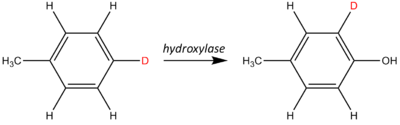
\includegraphics{nih.png}
\end{center}
Several hydroxylase enzymes are believed to follow NIH shift.\\

\textbf{Activated Sludge} is an important source of bacterial strains. The wastes from houses drains enter municipal drains which take them to a wastewater treatment plant. The wastewater is kept in a tank where sedimentation takes place. The liquid moves to another tank where additional particulates are removed. Then oxygen is bubbled through wastewater in the next tank, where bacterial growth takes place. Sludge contains a mixture of over 75000 bacterial species in the form of colonies. Out of these, there is a fairly good chance of finding a degrader for a particular organic compound. Industrial wastewater also contains different strains of bacteria, however, the process of treating wastes is closely guarded by most industries.\\

Phenolic compounds are environmental pollutants because of their widespread use and potential toxicity to higher organisms. p-Cresol is used in disinfectants and fumigants, in the manufacture of synthetic resins, in photographic developers, and in explosives. p-Cresol is highly toxic, corrosive, causes nervous system depression, affects lungs, liver, kidneys and heart. It also causes skin burns, respiratory tract irritation and has reproductive and teratogenic effects. p-Cresol is listed as a priority pollutant by the U.S. Environmental Protection Agency. Bioremediation is the most cost-effective method for complete destruction of organic pollutants like p-cresol.
\end{document}